% Part 6: RUI
\subsection{Cost plot}
\begin{frame}{Cost, efficiency, and false positive rate: 2 convolutionial layers}
   \centering
   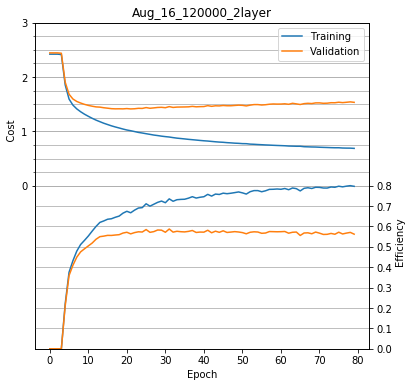
\includegraphics[width=0.45\linewidth]{images/CNN_2Layer_Cost.png}
   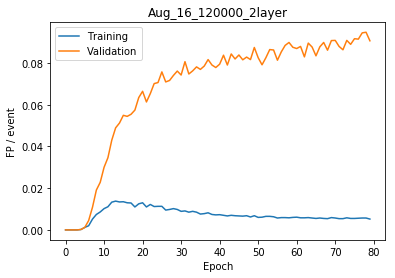
\includegraphics[width=0.45\linewidth]{images/CNN_2Layer_FalsePositive.png}

\end{frame}

\begin{frame}{Cost, efficiency, and false positive rate: 3 convolutionial layers}
   \centering
   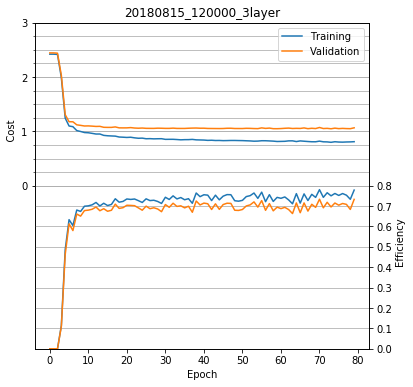
\includegraphics[width=0.45\linewidth]{images/CNN_3Layer_Cost.png}
   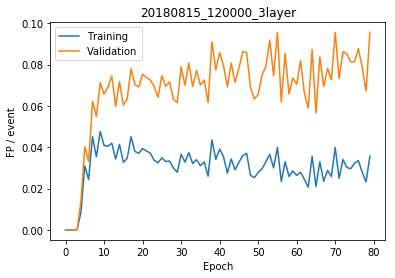
\includegraphics[width=0.45\linewidth]{images/CNN_3Layer_FalsePositive.png}

\end{frame}
\subsection{Prediction plots}

\begin{frame}{Compare predictions with targets (3 convolutional layers)}
  \begin{columns}[c]
    \column{.5\textwidth}
        \begin{center}
            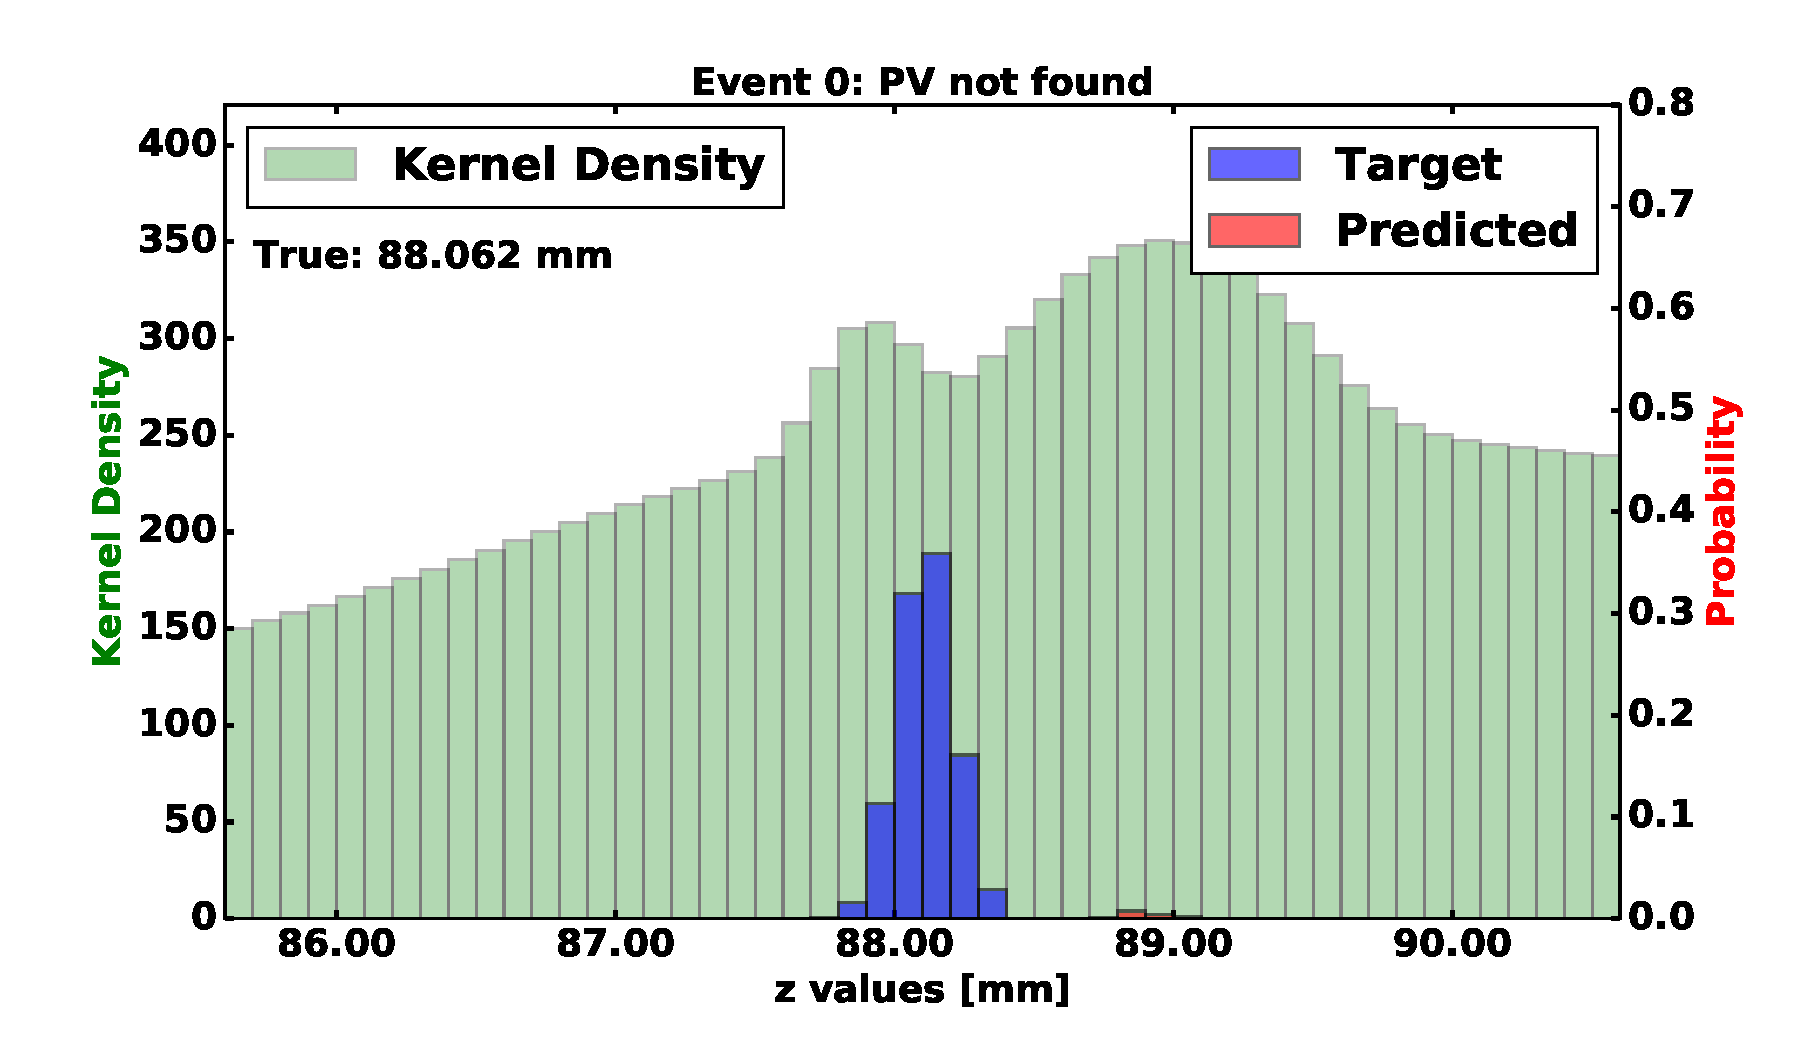
\includegraphics[width=1\textwidth,height=0.45\textwidth, trim=18 0 18 0]{images/120000_3layer_00.pdf}
    
            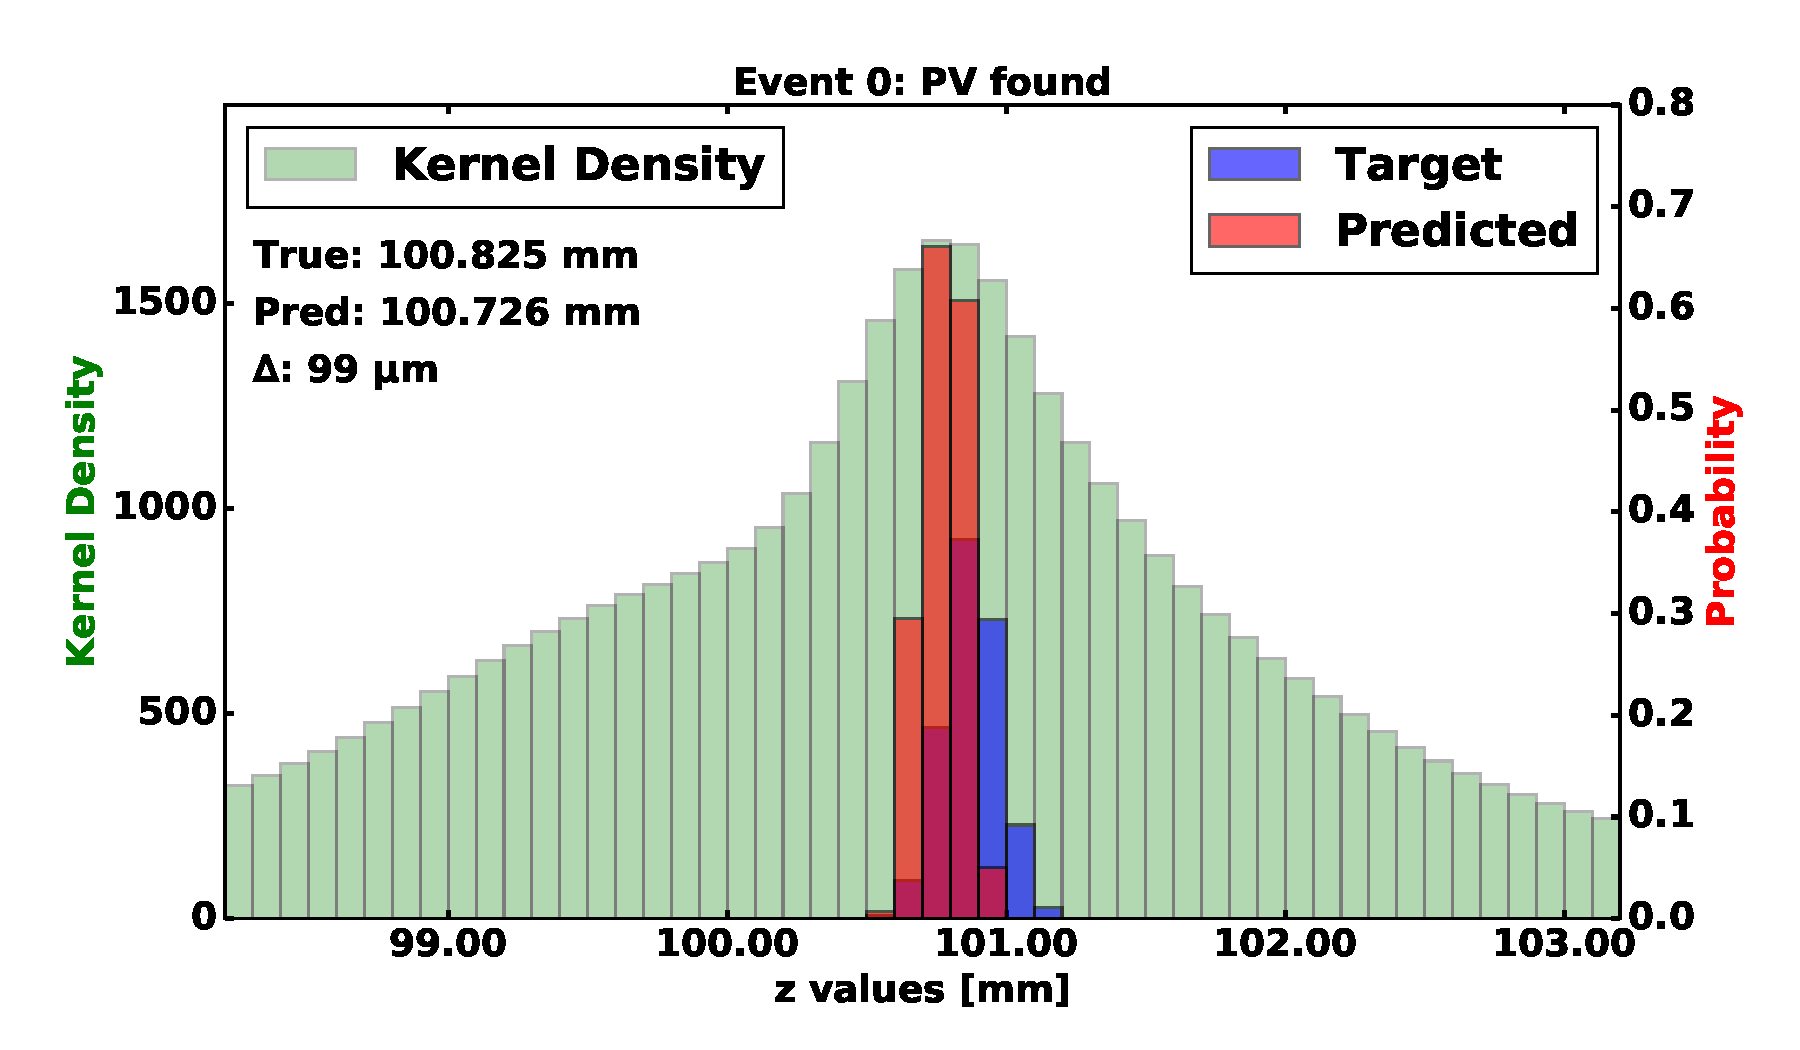
\includegraphics[width=1\textwidth, height=0.45\textwidth,trim=18 0 18 0]{images/120000_3layer_01.pdf}

        \end{center}
    \column{.5\textwidth}
        \begin{center}
           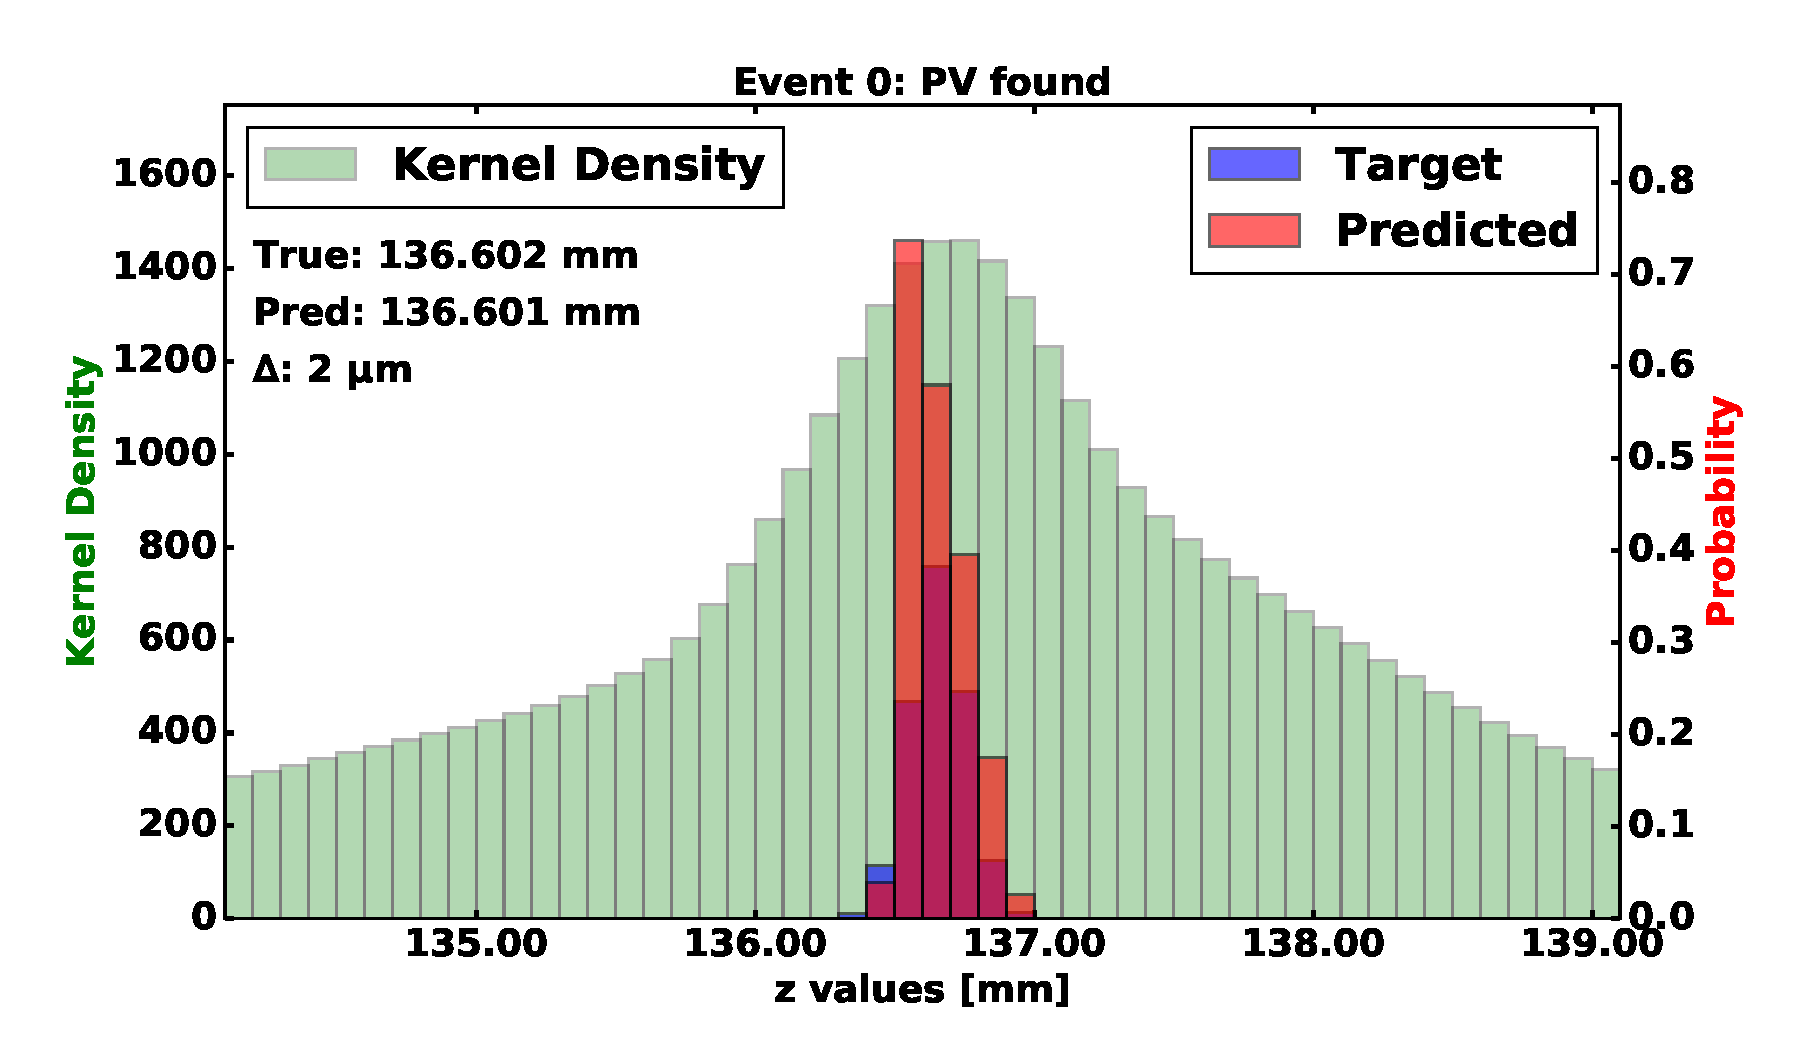
\includegraphics[width=1\textwidth, height=0.45\textwidth, trim=18 0 18 0]{images/120000_3layer_02.pdf}
    
           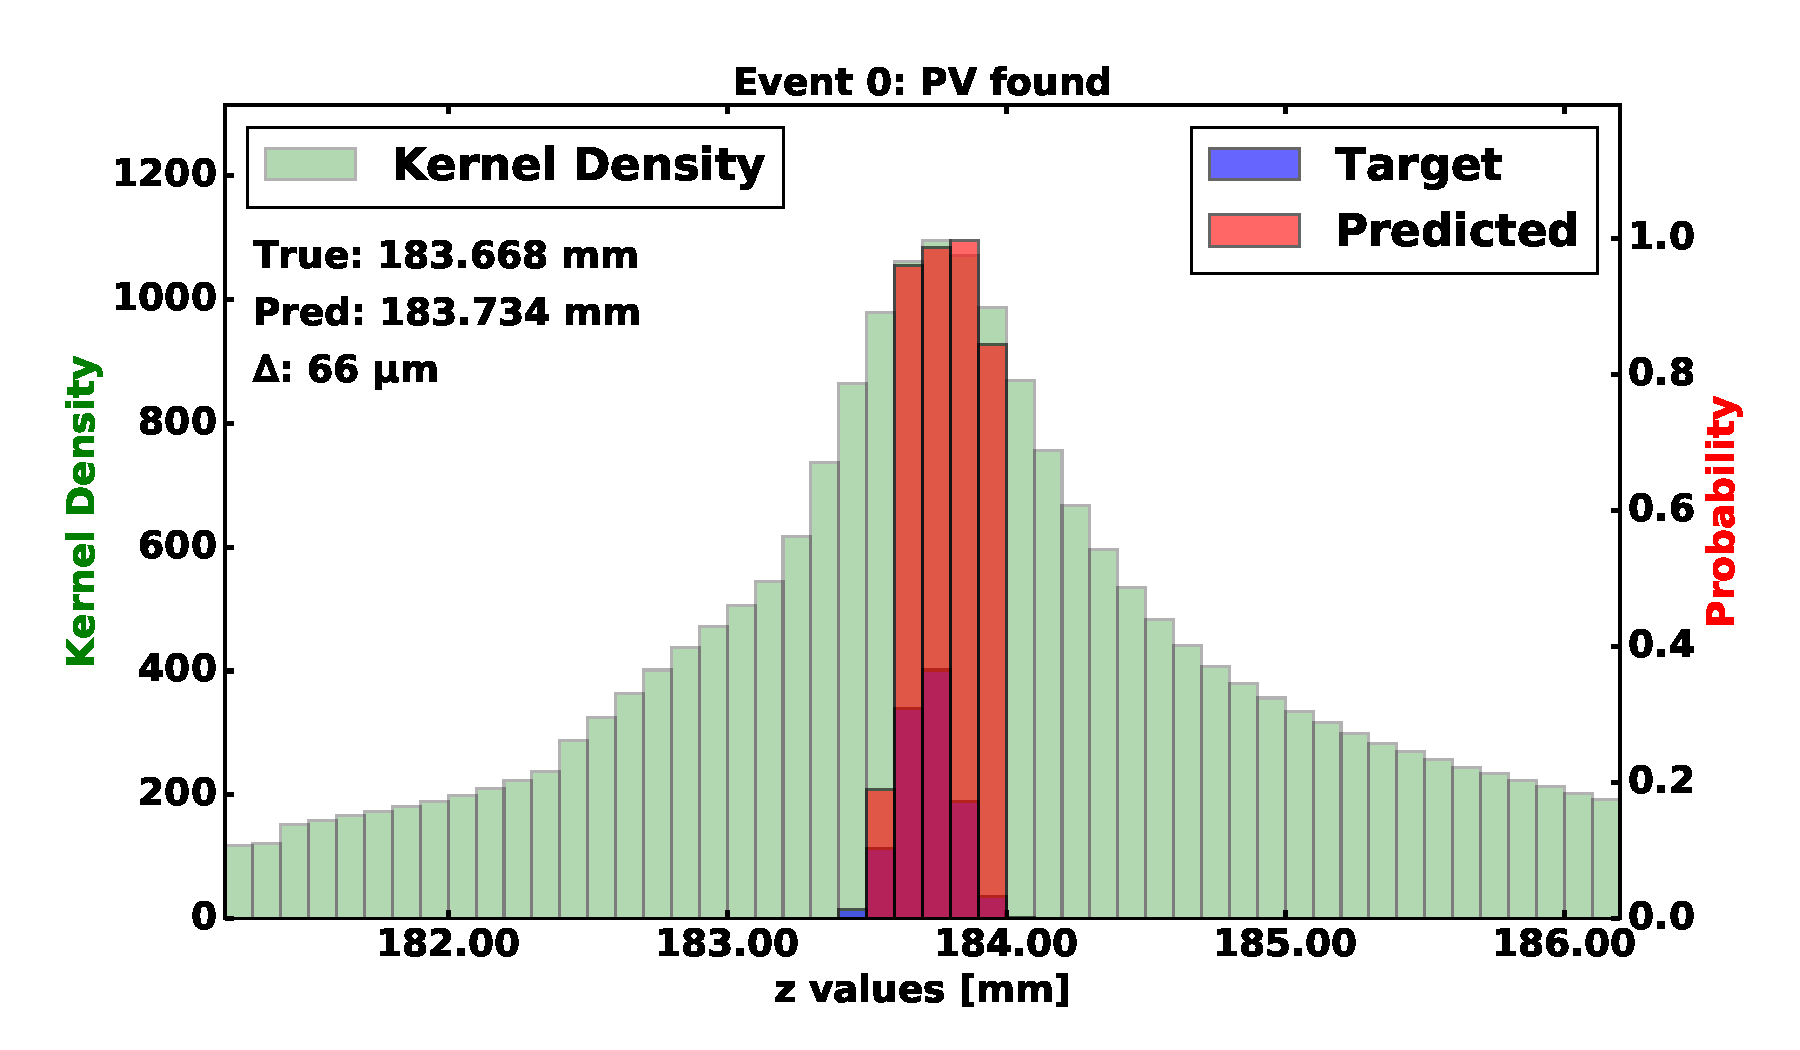
\includegraphics[width=1\textwidth, height=0.45\textwidth, trim=18 0 18 0]{images/120000_3layer_03.pdf}
       \end{center}
  \end{columns}
\end{frame}


\begin{frame}{Compare predictions with targets (3 convolutional layers)}
  \begin{columns}[c]
    \column{.5\textwidth}
        \begin{center}
            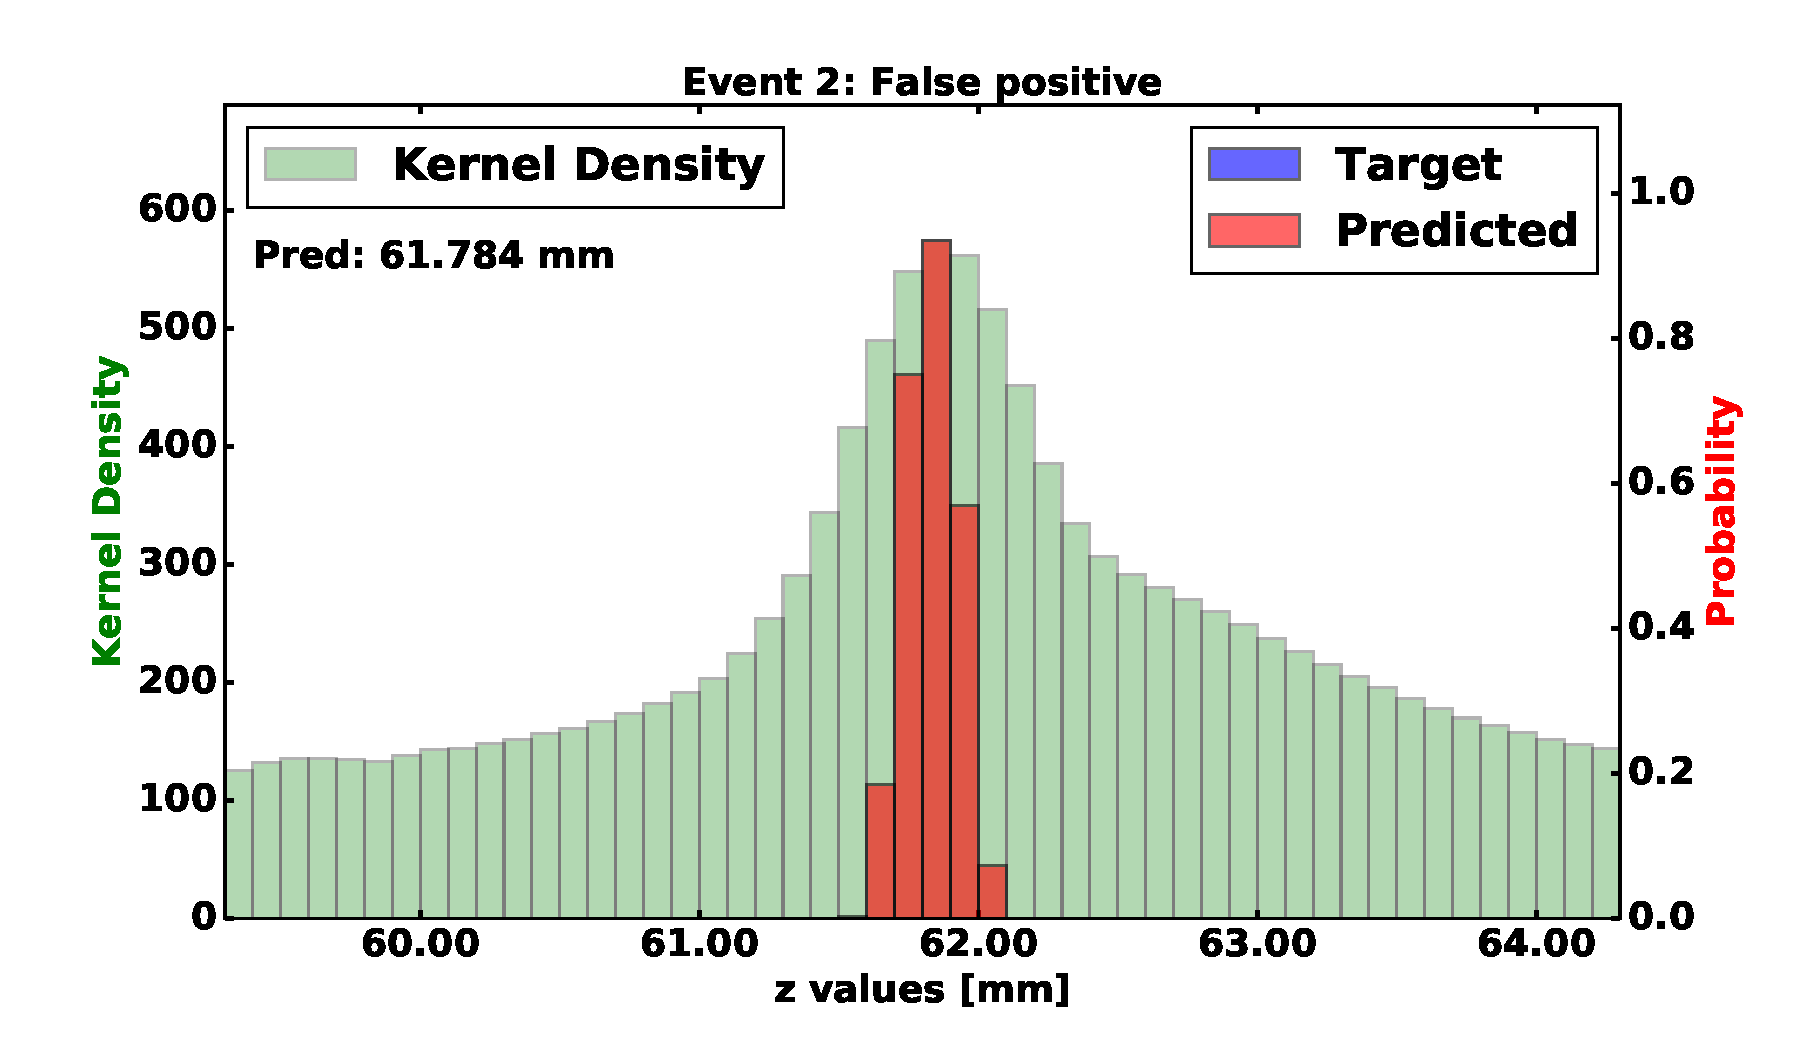
\includegraphics[width=1\textwidth,height=0.45\textwidth, trim=18 0 18 0]{images/120000_3layer_12.pdf}
    
            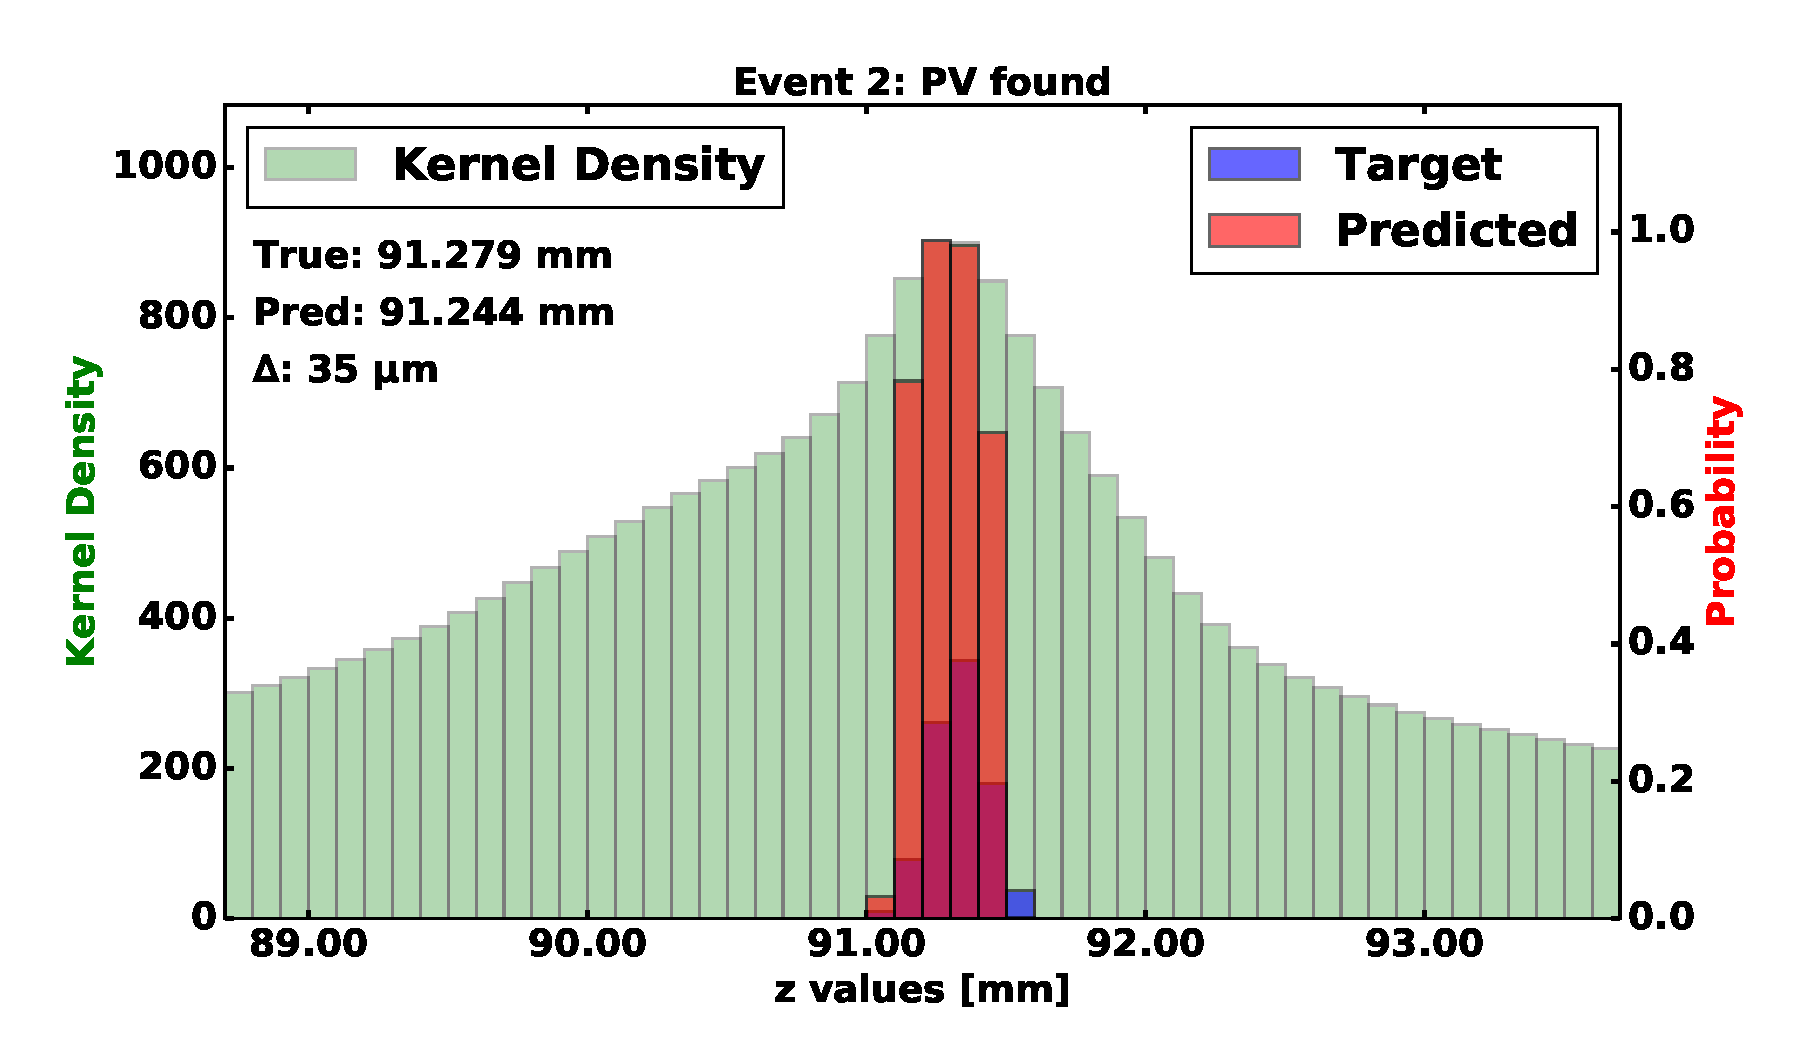
\includegraphics[width=1\textwidth, height=0.45\textwidth,trim=18 0 18 0]{images/120000_3layer_13.pdf}

        \end{center}
    \column{.5\textwidth}
        \begin{center}
           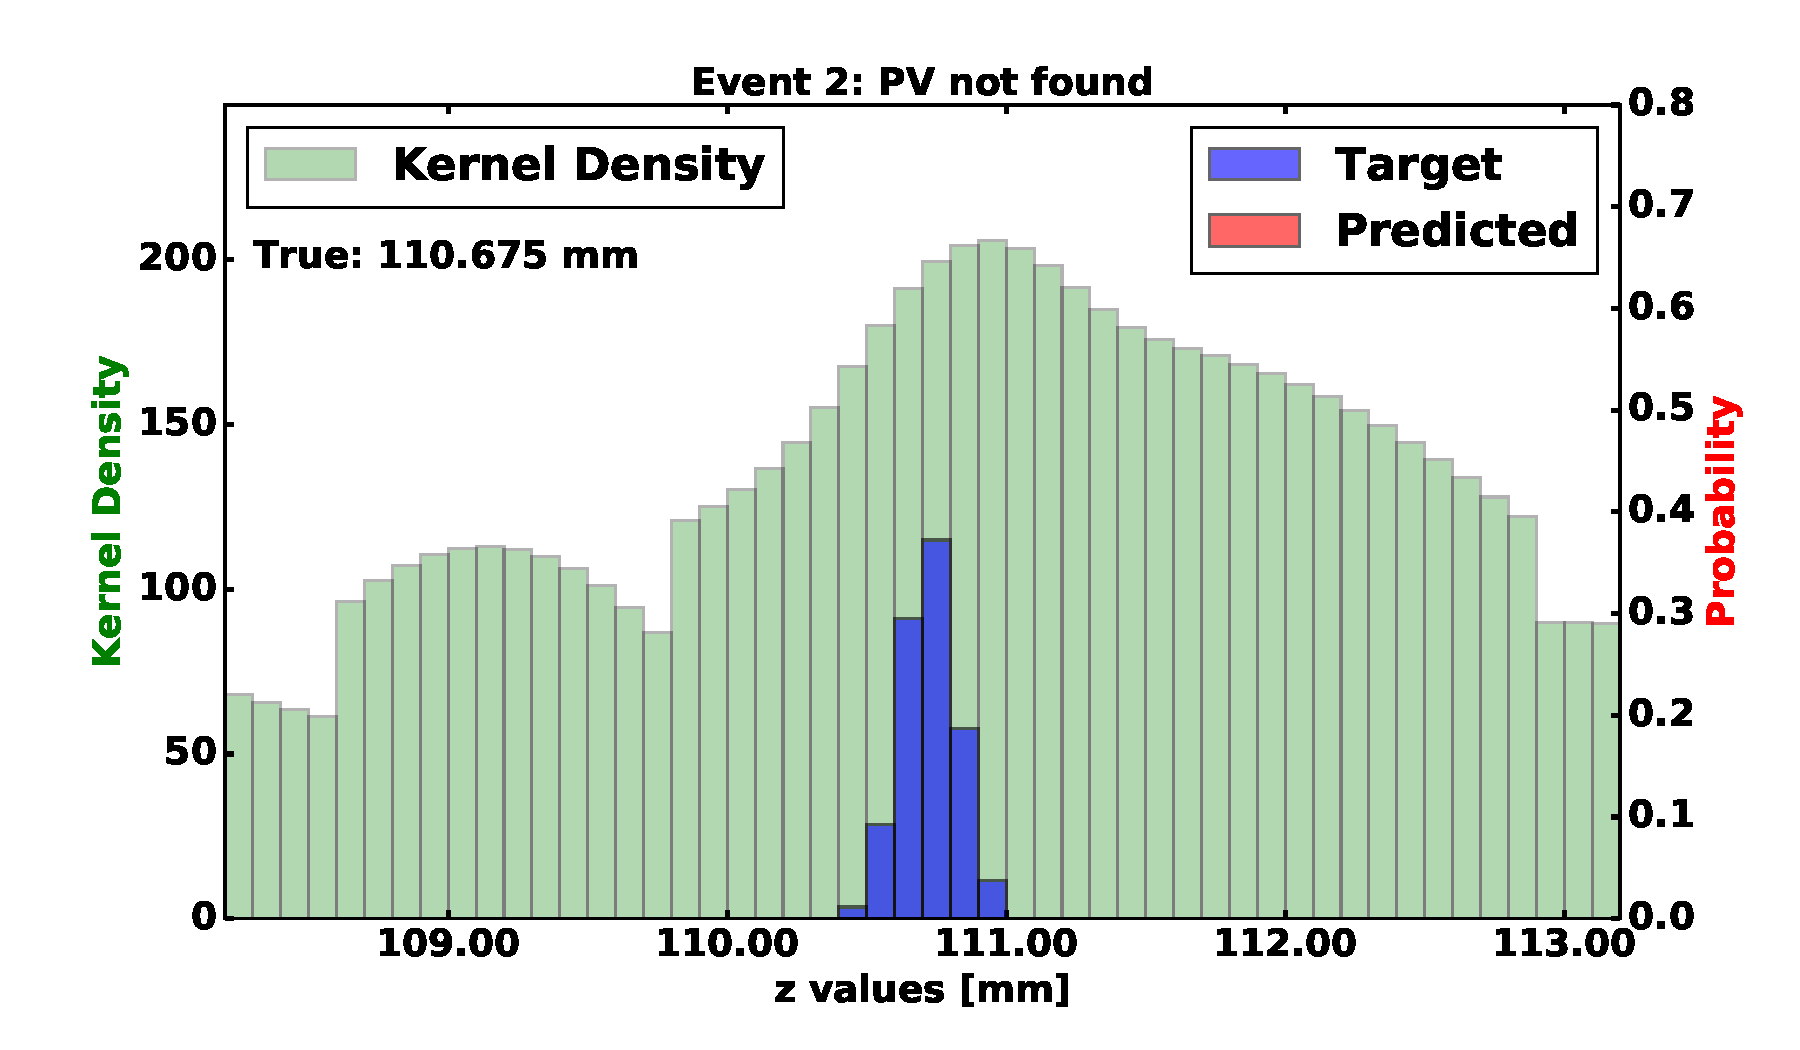
\includegraphics[width=1\textwidth, height=0.45\textwidth, trim=18 0 18 0]{images/120000_3layer_14.pdf}
    
           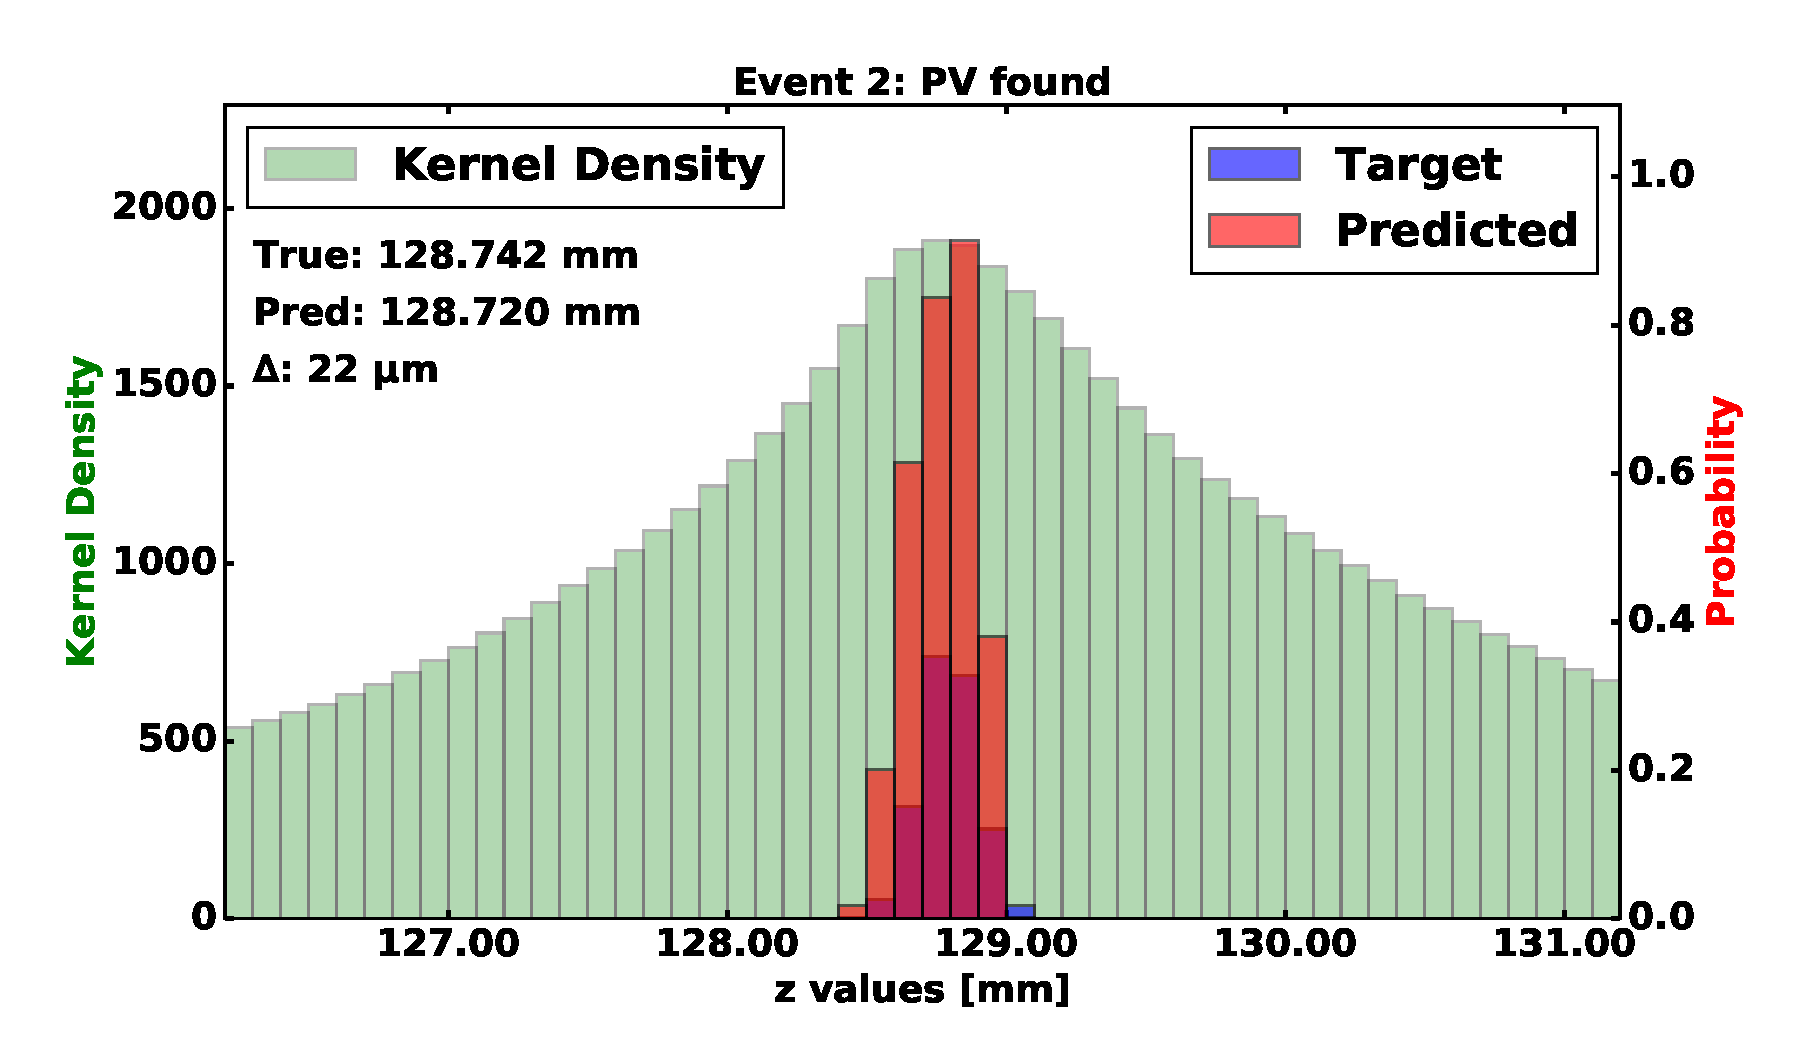
\includegraphics[width=1\textwidth, height=0.45\textwidth, trim=18 0 18 0]{images/120000_3layer_15.pdf}
       \end{center}
  \end{columns}
\end{frame}





% Part 7: RUI
\subsection{Quantitative results}
\begin{frame}{Efficiencies and false positive rates}
\begin{table}[]
\centering
\begin{tabular}{cccc}
parameter & 2 CVN Layers &
3 CVN Layers & 4 CVN Layers \\ [0.3em]

$\epsilon \textrm{(Efficiency)}
 = \frac{\mbox{TP}}{\mbox{TP} + \mbox{FN}} $
&  $ \approx 58\% $  & $ \approx 70\% $ & $ \approx 75\% $ \\ [0.3em]
$ \textrm{False Positive rate}
 = \frac{\mbox{FP}}{\mbox{number of events}} $
 &  $\approx 0.07 $ & $\approx 0.08 $  & $ \approx 0.13 $ \\
 \end{tabular}
\end{table}
 \vskip -0.05in
  \begin{table}[]
      \centering
      \begin{tabular}{c|cc}
         & Found & Not found \\ \midrule
         Real PV & True positive & False negative\\
         Not a real PV & False positive & True negative
      \end{tabular}
  \end{table}
  \vskip -0.15in
  \begin{block}{True Positive}
    \begin{itemize}
    	\item search $ \pm 5 $ bins ($ \pm 500 \mu $m) around a real PV
    	\item at least 3 (4) bins with predicted probability
    	   $ > 1\% $ and 
    	   integrated probability $ > 20\%$.
    \end{itemize}

    \end{block}
    \begin{block}{False Positive}
    \begin{itemize}
        \item
           at least 3 (4) bins with individual probabilities $ > 1\% $ and
          integrated probability $ > 20\%$.
        \item 
        no real PV within $ \pm 5 $ bins ($ \pm 500 \mu $m) of that cluster.
    \end{itemize}
  \end{block}
\end{frame}

\subsection{Asymmetric loss}
\begin{frame}{Asymmetric loss}
    \centerline{
        \begin{minipage}[t]{1.1\textwidth}
            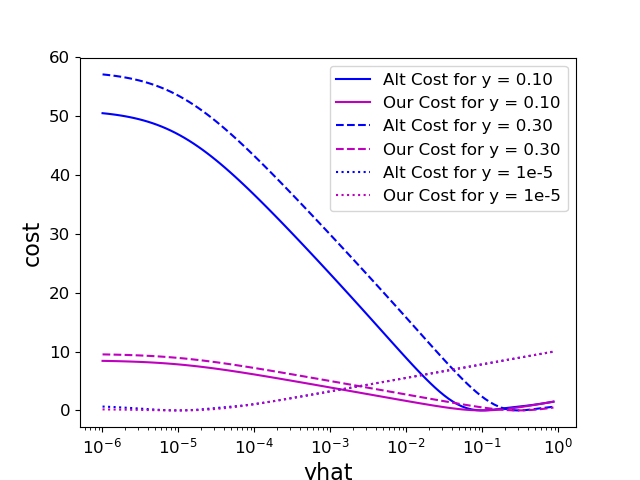
\includegraphics[width=.33\textwidth, clip, trim=10 0 40 0]{images/AltCostPlot_181015} 
            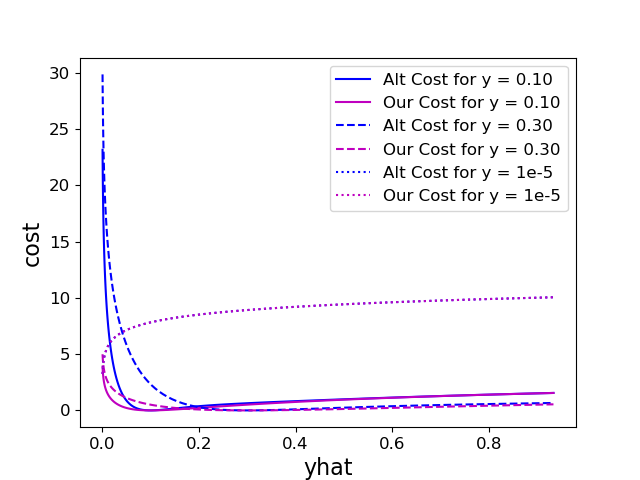
\includegraphics[width=.33\textwidth, clip, trim=10 0 40 0]{images/AltCostPlot_181015_linear} 
            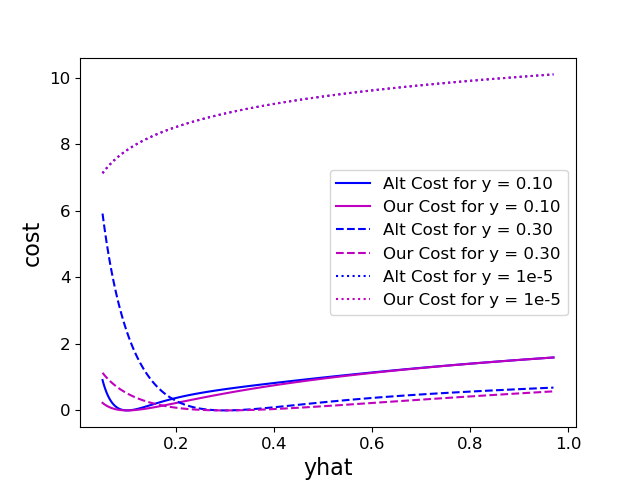
\includegraphics[width=.33\textwidth, clip, trim=10 0 40 0]{images/AltCostPlot_181015_linearA} 
        \end{minipage}
    }
\end{frame}

\subsection {New quantitative results}
\begin{frame}{Efficiencies and false positive rates, cont.}
\begin{table}[]
\centering
    {\Large With masking} \\
    \vspace{.5em}
\begin{tabular}{cccc}
    parameter & 3 CVN Layers & 4 CVN Layers & 4 CVN Layers \\
              &              &              & (asymmetric loss) \\ [0.3em]
    $ \epsilon \textrm{(Efficiency)} = \frac{\mbox{TP}}{\mbox{TP} + \mbox{FN}} $ &  $ \approx 80\% $  & $ \approx 82\% $ & $ \approx 92\% $ \\ [0.7em]
    $ \textrm{False Positive rate} = \frac{\mbox{FP}}{\mbox{number of events}} $ &  $\approx 0.03  $  & $\approx 0.03  $ & $ \approx 0.18 $ \\
 \end{tabular}
\end{table}
\end{frame}
